\documentclass[12pt]{article}
\usepackage{graphicx} % Required for inserting images
\usepackage{hyperref}
\usepackage{makecell}
\usepackage{makeidx}
\usepackage{eurosym}
\usepackage{fancyhdr}
\usepackage{titlesec}
\usepackage{longtable}
\newcommand{\firstPage}{
    \thispagestyle{empty}
    \begin{figure}
    \centering
    
\includegraphics[scale=0.7]{Swellfish_logo.png}
    \end{figure}
    \author{
        \date{}
        \href{mailto://swellfish14@gmail.com}{swellfish14@gmail.com} \\
    } 
} 
\usepackage{hyperref}
\usepackage{array}
\usepackage{tabularx}
\usepackage{adjustbox}

\newcounter{verscount}
\setcounter{verscount}{0}
\newcommand{\addversione}[5]{
	\ifdefined\setversione
		\setversione{#1}
	\else\fi
	\stepcounter{verscount}
	\expandafter\newcommand%
		\csname ver\theverscount \endcsname{#1&#2&#3&#4&#5}
}

\newcommand{\listversioni}{
	\ifnum\value{verscount}>1
		\csname ver\theverscount \endcsname
		\addtocounter{verscount}{-1}
		\\\hline
		\listversioni
	\else
		\csname ver\theverscount \endcsname\\\hline
	\fi
}

\newcommand{\makeversioni}{
	\begin{center}
		\begin{tabularx}{\textwidth}{|c|c|X|X|X|}
		\hline
		\textbf{Versione} & \textbf{Data} & \textbf{Redattore} & \textbf{Verificatore} & \textbf{Descrizione} \\
		\hline
		\listversioni
		\end{tabularx}
	\end{center}
	\clearpage
}

\fancypagestyle{genericDocstyle}{
	\pagestyle{fancy}
	\lhead{
\includegraphics[width=1cm]{Swellfish_logo.png}}
	\rhead{Norme di progetto}
}

%\hypersetup{colorlinks=true,urlcolor=blue}

%\newcommand{\tableContent}{

	%{
		%\hypersetup{linkcolor=black}
		%\tableofcontents
	%}
%}
\graphicspath{ {../templates/img/} }

\begin{document}
\setcounter{tocdepth}{4}
\setcounter{secnumdepth}{4}
\title{Analisi dei Requisiti}

\firstPage
\pagebreak

\maketitle

\begin{center}
    \begin{tabular}{r | l}
		\multicolumn{2}{c}{\textit{Informazioni}}\\
		\hline
		
			\textit{Redattori} &
			[Davide Porporati, Elena Marchioro, Francesco Naletto]\makecell{}\\

			\textit{Revisori} &
			[Jude Vensil Braceros]\makecell{}\\
			\textit{Responsabili} &
			[Andrea Veronese]\makecell{}\\
		      \textit{Uso} & 
                [Esterno]\makecell{}\\
    \end{tabular}
\end{center}

\begin{center}
    \textbf{Descrizione}\\
	File contenente l'analisi dei requisiti necessaria per la realizzazione del progetto. 
\end{center}

\pagebreak

\addversione{0.0.0}{24/04/2023}{Andrea Veronese}{Davide Porporati}{Creata struttura di base del documento}
\addversione{0.0.1}{24/04/2023}{Davide Porporati, Elena Marchioro, Francesco Naletto}{Jude Vensil Barceros}{Aggiunti casi d'uso di base}
\addversione{0.0.2}{26/04/2023}{Davide Porporati, Elena Marchioro, Francesco Naletto}{Jude Vensil Barceros}{Aggiunta nuovi casi uso come da capitolato Lumos Minima}
\addversione{0.0.3}{03/05/2023}{Elena Marchioro, Francesco Naletto, Jude Vensil Braceros}{Andrea Veronese}{Ristrurati casi d'uso in vista del primo diario di bordo}
\addversione{0.0.4}{09/05/2023}{Andrea Veronese, Francesco Naletto, Jude Vensil Braceros}{Claudio Giaretta}{Aggiunti ulteriori casi d'uso}
\addversione{0.0.5}{17/05/2023}{Andrea Veronese, Claudio Giaretta, Jude Vensil Braceros}{Davide Porporati}{Modificati casi d'uso su indicazione di Imola Informatica}
\addversione{0.0.6}{30/05/2023}{Davide Porporati}{Claudio Giaretta}{Inserite le immagini UML}
\addversione{0.1.0}{07/06/2023}{Claudio Giaretta}{Francesco Naletto}{Aggiornate le immagini UML e verificato intero documento}
\addversione{1.0.0}{18/06/2023}{Claudio Giaretta}{Francesco Naletto}{Aggiornato a versione 1.0.0}
\addversione{1.0.1}{18/06/2023}{Claudio Giaretta}{Andrea Veronese}{Aggiunti vincoli di compatibilità con browser}
\addversione{1.0.2}{01/09/2023}{Davide Porporati, Elena Marchioro}{Andrea Veronese}{Aggiornati UC in base alla consegna della PB}
\addversione{2.0.0}{12/09/2023}{Davide Porporati, Elena Marchioro}{Andrea Veronese}{Revisionato e verificato il documento per la consegna della PB}
\makeversioni

\pagebreak
\tableofcontents

\pagebreak

\graphicspath{ {./UML/images/} }

\section{Introduzione}
Lo scopo di questo documento è quello di raccogliere i risultati dell'attività di analisi dei requisti, includendo la descrizione dei casi d'uso del software e i requisiti necessari per la sua realizzazione.
Questa analisi nasce dalla necessità di dimostrare di aver capito a fondo i requisiti del problema e le aspettative della soluzione che il nostro gruppo andrà a proporre.
I casi d'uso analizzati in seguito, dovranno essere tenuti in considerazione durante tutte le fasi di progettazione, verifica e validazione.

\subsection{Riferimenti}
Questo documento contiene un'analisi tecnica dei requisiti necessari allo sviluppo del software per il capitolato C2 Lumos Minima.

I documenti in cui vengono specificati i requisiti sono i seguenti:
\begin{itemize}
	\item Capitolato d'appalto C2
	\item Norme di progetto
	\item Verbale dell'incontro conoscitivo con Imola del 14/03/2023
	\item Verbale dell'incontro per l'approfondimento dei requisiti con Imola del 21/04/2023
	\item Verbale dell'incontro per la revisione dei casi d'uso con Imola del 16/05/2023
\end{itemize}

Mentre i documenti che ci forniscono un'indicazione su come fare sono i seguenti:
\begin{itemize}
	\item Slide analisi requisiti - T06, prof. Vardenega
	\item Slide diagrammi d'uso - Diagrammi e Use Case, prof. Cardin
\end{itemize}

\section{Descrizione del prodotto}
L'azienda Imola Informatica propone lo sviluppo di una "$webapp$" che consente la gestione automatica o manuale degli impianti di illuminazione pubblica "$smart$", ovvero dotati di sensori in grado di rilevare la presenza di persone o veicoli in transito.
Lo scopo del progetto è quello di fornire una piattaforma che grazie all'automazione permette di ridurre i consumi elettrici e aumentare la sicurezza stradale dei luoghi in cui verrà impiegata.
Il funzionamento di tale sistema avviene secondo delle fasi ben precise:
\begin{itemize}
	\item l'illuminazione viene impostata ad un livello standard, ovvero un numero compreso tra 0 (spento) e 10(luminosità massima)
	\item Se un sensore rileva un veicolo o una persona, aumenta la luminosità di tutti i lampioni dell'area ad un livello prefissato
	\item Viene fatto trascorrere un intervallo temporale predefinito, nell'ordine di alcuni minuti
	\item Se al termine dell'intervallo stabilito non ci sono nuovi rilevamenti da parte dei sensori, la luminosità viene abbassata, come descritto nel primo punto del funzionamento del sistema, al livello pre-rilevamento.
\end{itemize}
Oltre al funzionamento automatico il capitolato prevede la possibilità di un funzionamento manuale. \\
Questa modalità deve permettere all'amministratore di sistema di aumentare o ridurre a piacimento la luminosità in una data area, senza che ci sia un effettivo rilevamento.

\subsection{Parti del prodotto}
Il sistema software sarà composto dalle seguenti unità:
\begin{itemize}
	\item webapp, ovvero la pagina web che permette di gestire la aree illuminate
	\item interfacciamento con i lampioni e con i sensori, che avverrà tramite chiamate api-rest o client mqtt.
	\item schermata di login/logout, per consentire l'accesso al sistema solamente ai soggetti autorizzati
	\item tracciamento dei guasti
	\item schermata per aggiungere,modificare o eliminare lampioni/sensori o intere aree illuminate
	\item manuale d'uso
\end{itemize}
Il termine "WebApp" si riferisce all'insieme dei seguenti componenti del sistema:
\begin{itemize}
	\item Frontend: Dashboard accessibile via web che permette di interagire graficamente con il sistema
	\item Backend: Sistema di comunicazione e interazione con i dispositivi IoT utilizzati per gestire la luminosità di un'area. Include anche tutti gli strumenti necessari per manipolare i dati di interesse dell'applicazione, come i lampioni, i sensori e le aree.
	\item Database: sistema usato per salvare e gestire dati strutturati di interesse per l'applicazione.
\end{itemize}

\subsection{Caratteristiche degli utenti}
Il capitolato prevede la presenza di due categorie distinte di utenti, ovvero l'amministratore di sistema e il manutentore. \\
Con Imola Informatica è stato concordato che entrambe le categorie di utenti riceveranno le credenziali direttamente dal gestore dell'impianto.
L'utente che ricoprirà il ruolo di amministratore può eseguire le seguenti operazioni:
\begin{itemize}
	\item Accedere alla dashboard
	\item Aumentare manualmente l'intensità luminosa di una o più aree
	\item Aggiungere, modificare e rimuovere lampioni in un'area predefinita
	\item Aggiungere, rimuovere o modificare le aree di illuminazione
	\item Tracciare le aree guaste e inserirle in un apposito elenco che funge da storico dei malfunzionamenti
\end{itemize}
Il SuperAmministratore potrà eseguire le seguenti operazioni:
\begin{itemize}
	\item tutte le operazioni consentite all'amministratore
	\item fornire le credenziali ai nuovi amministratori di sistema
\end{itemize}
Il manutentore godrà invece di permessi più limitati, infatti potrà eseguire le seguenti azioni:
\begin{itemize}
	\item consultare la lista degli impianti guasti
	\item rimuovere un impianto guasto dopo aver effettuato la manutenzione
\end{itemize}
\subsection{Vincoli e preferenze}

\subsubsection{Vincoli Tecnologici}
L'azienda proponente non ha imposto vincoli teconologici, ma ha dato dei suggerimenti da considerare:
\begin{itemize}
	\item Utilizzare framework open-source e ben noti, che non comportino il pagamento di canoni mensili o di licenze
	\item L'interfacciamento con i sensori o con i lampioni potrà avvenire tramite api-rest oppure tramite un broker mqtt come "$Mosquito$"
	\item L'applicazione dovrà essere compatibile con i seguenti browser: 
	\begin{itemize}
		\item \textbf{Opera}: versione 110 o superiore
		\item \textbf{Safari}: versione 16.0 o superiore
		\item \textbf{Chrome}: versione 110 o superiore
		\item \textbf{Firefox}: versione 110 o superiore
		\item \textbf{Edge}: versione 95 o superiore
	\end{itemize}
\end{itemize}

\subsubsection{Vincoli di consegna}
Per il completamento del progetto il proponente richede che le seguenti condizioni siano soddisfatte:
\begin{itemize}
	\item Soddisfacimento di tutti i requisiti obbligatori descritti nel capitolato
	\item test che dimostrino il corretto funzionamento delle funzionalità previste, con una percentuale di superamento \begin{math}\geq 80\% \end{math}, correlata da appositi report
	\item webapp completa, dotata di UI responsive
	\item documentazione su scelte implementative e progettuali effettuate,\\ con relativo registro delle motivazioni, dei problemi incontrati e delle soluzioni adottate per superarli.
\end{itemize}

\subsubsection{Vincoli prestazionali}
Il sistema suppone di utilizzare istanze di massimo 1GB di memoria e 2 CPU.

\subsubsection{Vincoli Opzionali}
\begin{itemize}
	\item Cifratura di tutte le comunicazioni tra app e server
	\item Vincoli di tempo permettendo, fornire un'analisi del carico massimo di sistema e dei servizi cloud più adatti ad hostare il sistema
\end{itemize}


\section{Casi d'uso}

\subsection{Attori primari}
Utente: persona con apposite credenziali e permessi che può accedere ad aree diverse del sistema ed eseguire operazioni differenti
Gli utenti vengono suddivisi nelle seguenti sottocategorie, ognuna delle quali ha dei privilegi e delle azioni eseguibili specifiche.
\begin{itemize}
	\item SuperAdmin: utente dotato dei massimi privilegi. Può fornire le credenziali ad altri amministratori e idealmente corrisponde alle società che utilizzano Lumos Minima
	\item Admin: Utente amministratore standard. Può effettuare tutte le operazioni previste dal sistema.
	\item Manutentore: utente base che può accedere a funzionalità limitate, riguardanti solamente la manutenzione dei lampioni e la gestione dei guasti.
\end{itemize}
Dopo aver sviluppato il Poc e constatata la ristrettezza dei tempi per lo sviluppo della baseline architetturale, di comune accordo con l'azienda proponente è stato deciso di non implementare il manutentore come attore del sistema. Nonostante ciò il sistema di ticketing, accessibile anche dal manutentore, è stato comunque sviluppato poichè usato anche dall'amministratore.
\\

\end{itemize}

\subsection{Diagrammi dei casi d'uso}

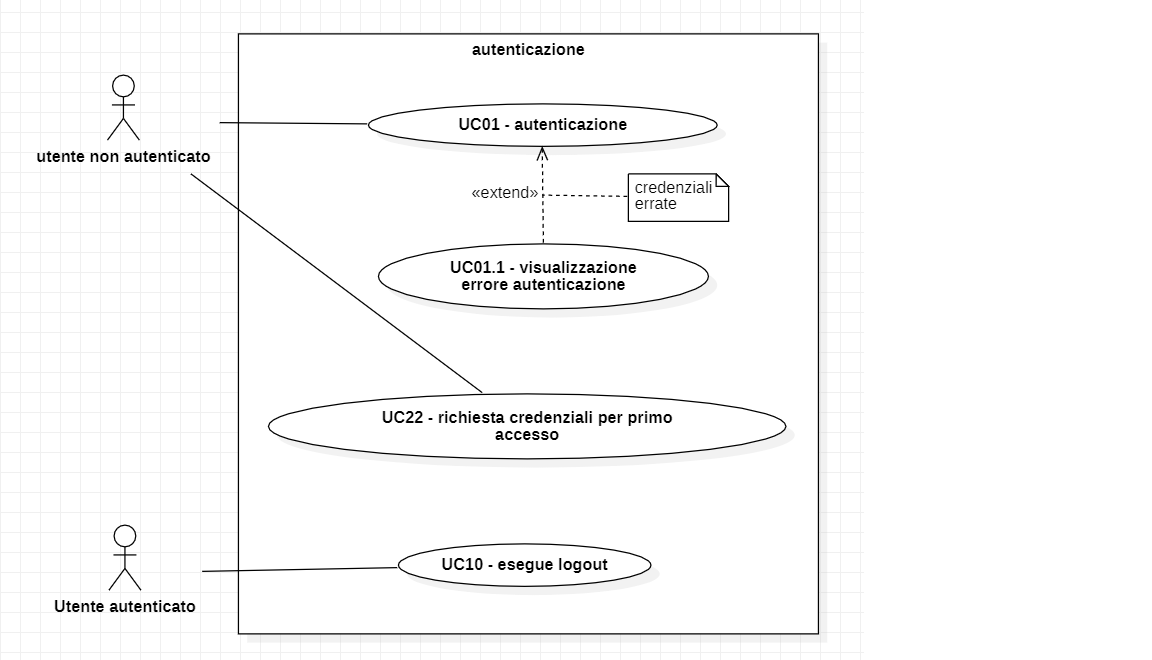
\includegraphics[scale=0.5]{autenticazione.png}

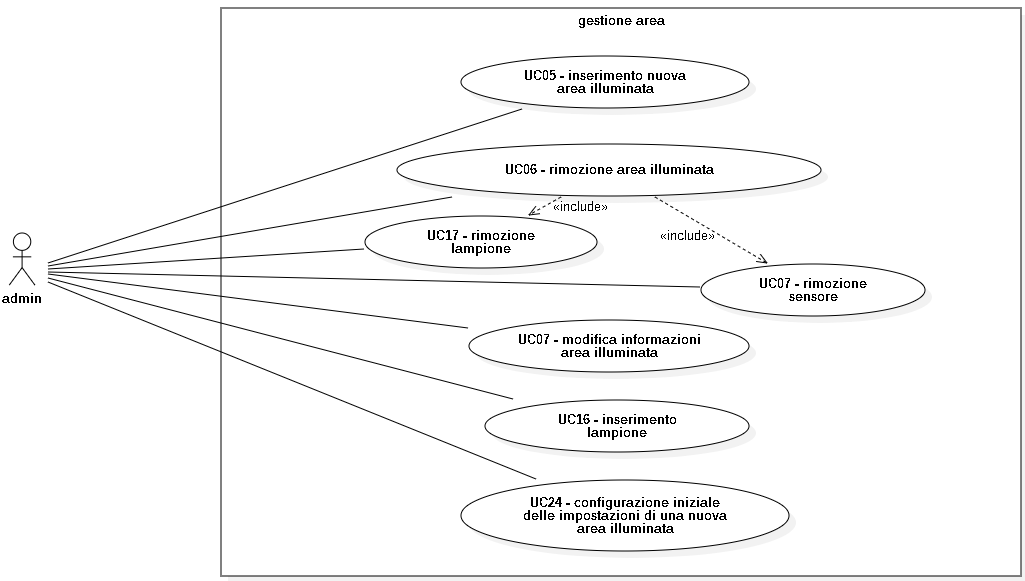
\includegraphics[scale=0.5]{gestione area.png}	

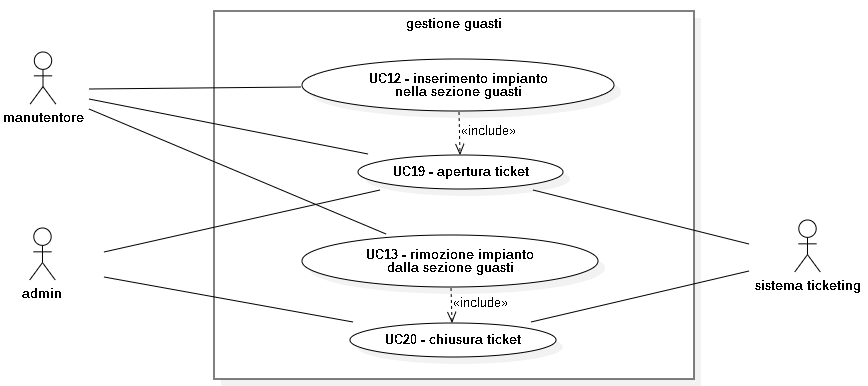
\includegraphics[scale=0.5]{gestione guasti.png}	

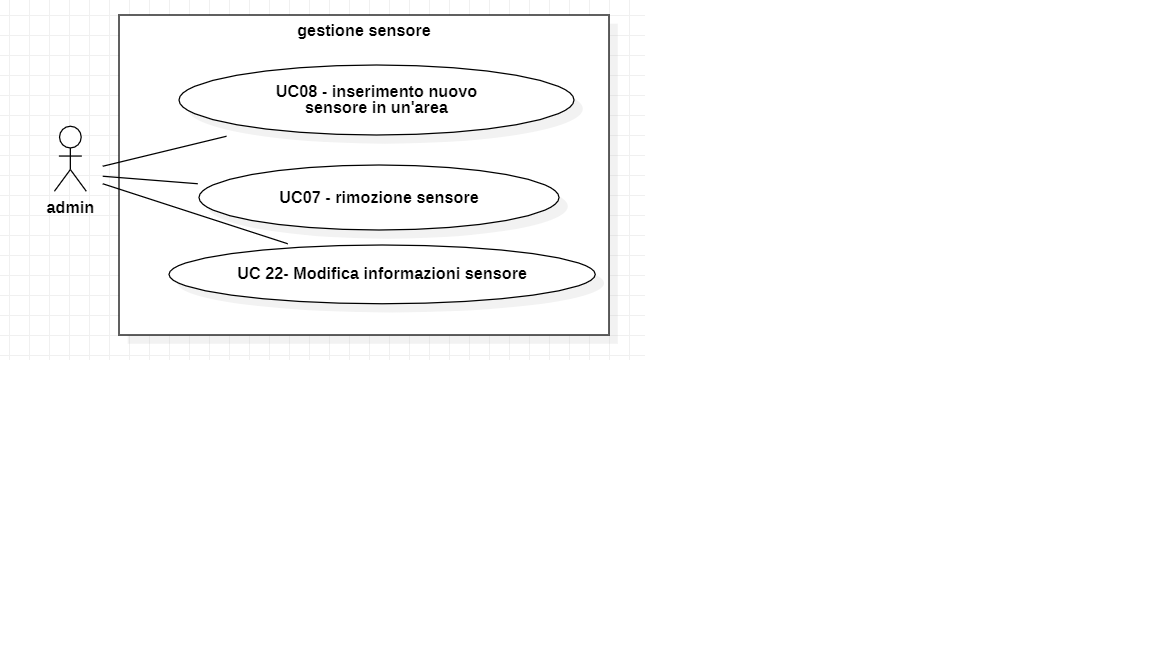
\includegraphics[scale=0.5]{gestione sensore.png}	

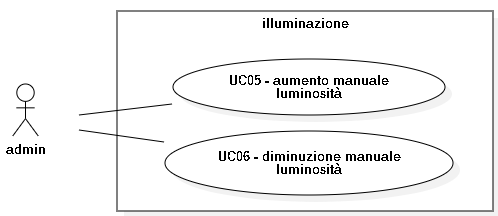
\includegraphics[scale=0.5]{illuminazione.png}	

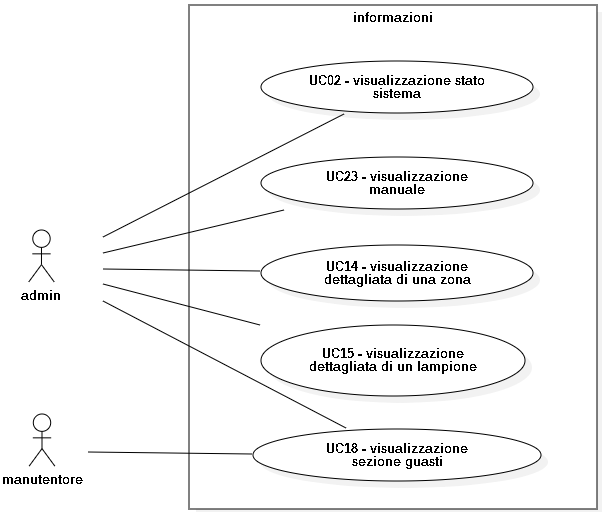
\includegraphics[scale=0.5]{informazioni.png}	

\pagebreak
\section{UC Obbligatori}

\subsection{UC01 - Accesso al sistema con credenziali}
\textbf{Tipologia: obbligatorio} \\
L'utente è in possesso delle credenziali ed è riconosciuto come amministratore, ma non ha ancora effettuato l'accesso.
\begin{itemize}
	\item Attori primari: SuperAdmin, Admin
	\item Precondizioni: l'amministratore vuole accedere al sistema per poterlo gestire, ma non è ancora loggato pur facendo parte del gruppo di utenti autorizzati.
	\item Postcondizioni: l'utente è riconosciuto dal sistema e può svolgere le consuete attività
\end{itemize}
\paragraph{Scenario Principale}
\begin{itemize}
	\item l'utente inserisce l'username
	\item l'utente inserisce la password
	\item l'utente riceve una conferma di avvenuto accesso e può operare nella dashboard
\end{itemize}
\paragraph{Estensioni} L'utente non è riconosciuto o non è presente nella lista dei soggetti autorizzati. Si rimanda allo "$UC21 $".

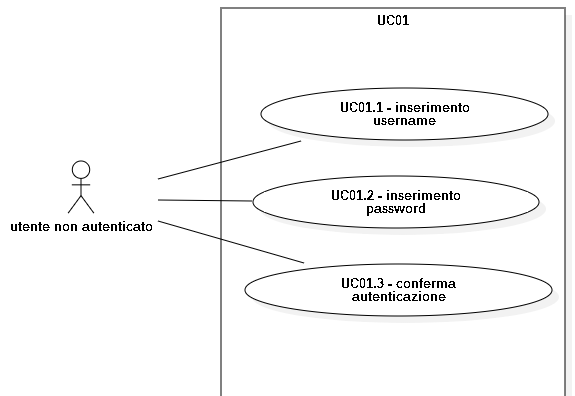
\includegraphics[scale=0.4]{UC01.png}

\subsection{UC02 - Visualizzazione stato sistema}
\textbf{Tipologia: obbligatorio} \\
L'utente autorizzato desidera avere una panoramica sullo stato del sistema.
\begin{itemize}
	\item Attori primari: SuperAdmin, Admin
	\item Precondizioni: l'utente è un amministratore e vuole avere una panoramica sulla luminosità del sistema e sullo stato operativo delle aree gestite
	\item Postcondizioni: la webapp fornisce queste informazioni
\end{itemize}
\paragraph{Scenario Principale}
\begin{itemize}
	\item l'amministratore si è loggato
	\item la webapp mostra la dashboard come landing page
\end{itemize}

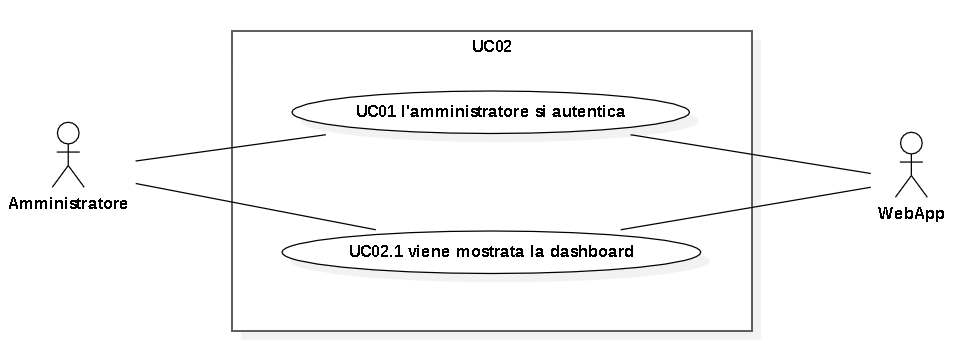
\includegraphics[scale=0.5]{UC02.png}

\subsection{UC03 - Aumento luminosità manuale}
\textbf{Tipologia: obbligatorio} \\
L'amministratore vuole aumentare la luminosità indipendentemente dal fatto che ci sia un rilevamento o meno.
\begin{itemize}
	\item Attori primari: SuperAdmin, Admin
	\item Precondizioni: gli amministratori vogliono aumentare manualmente la luminosità di un'area
	\item Postcondizioni:viene incrementata la luminosità dell'area dopo aver fatto trascorre un "tempo tecnico" necessario per la propagazione dei comandi a tutti i lampioni afferenti ad un'area specifica.
\end{itemize}
\paragraph{Scenario Principale}
\begin{itemize}
	\item l'utente accede alla dashboard
	\item l'utente seleziona una o più aree con cui operare
	\item il database fornisce gli indirizzi ip dei lampioni dell'area interessata
	\item l'utente incrementa manualmente la luminosità dell'area selezionata
\end{itemize}
\paragraph{Estensioni} In caso di guasto di sistema o mancanza di rete, l'amministratore comanda l'aumento della luminosità ma non vi è un incremento effettivo dopo aver fatto trascorrere il tempo tecnico prefissato.\\
Al termine di questo lasso di tempo, se non vi è un cambiamento nella luminosità del sistema, l'area viene inserita dall'amministratore nell'elenco dei guasti. 

\subsubsection{UC03.1 - Visualizzazione del messaggio d'errore}
\begin{itemize}
	\item Attore primario: SuperAdmin, Admin
	\item Precondizioni: L'attore primario ha tentato di aumentare la luminosità di una o più aree senza successo
	\item Post-condizioni: L'attore primario visualizza un messaggio recante un messaggio di errore
\end{itemize}

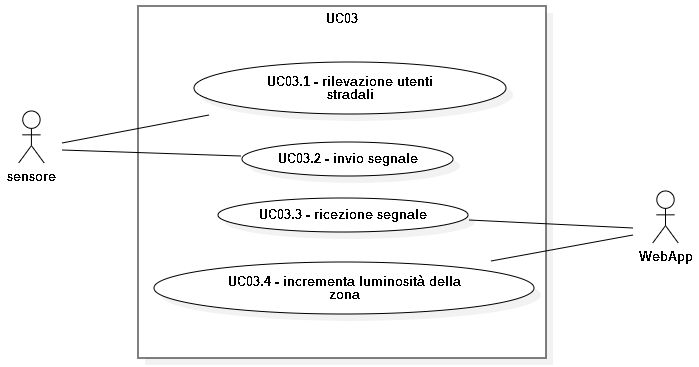
\includegraphics[scale=0.5]{UC03.png}

\subsection{UC04 - Diminuzione luminosità manuale}
\textbf{Tipologia: obbligatorio} \\
L'amministratore vuole diminuire la luminosità indipendentemente che ci siano rilevamenti di utenti stradali o meno.
\begin{itemize}
	\item Attori primari: SuperAdmin, Admin
	\item Precondizioni: gli amministratori vogliono diminuire manualmente la luminosità di un'area
	\item Postcondizioni: tutti i lampioni dell'area vedono una diminuzione della luminosità
\end{itemize}
\paragraph{Scenario Principale}
\begin{itemize}
	\item l'utente accede alla dashboard
	\item l'utente seleziona una o più aree con cui operare
 	\item il database fornisce gli indirizzi ip dei lampioni dell'area interessata
	\item l'utente decrementa manualmente la luminosità delle aree selezionate
\end{itemize}
\paragraph{Estensioni} Nel caso in cui si comandi una dimunuzione della luminosità in modalità manuale, ma il sensore non rileva un decremento effettivo della luminosità dopo aver fatto trascorrere il "tempo tecnico", si visualizza un messaggio di errore.
Al termine del tempo prefissato, se non ci sono stati cambiamenti di luminosità, il sistema può essere inserito nell'elenco dei guasti dall'amministratore.

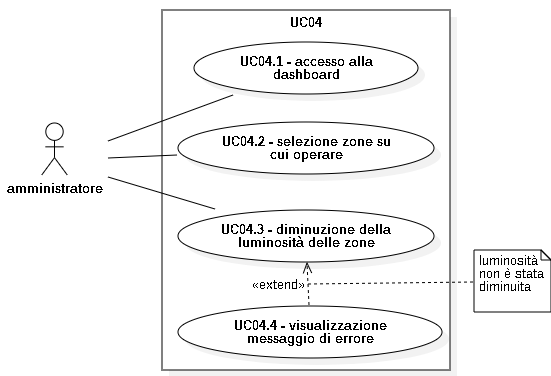
\includegraphics[scale=0.5]{UC04.png}

\subsection{UC05 - Inserimento nuova area illuminata}
\textbf{Tipologia: obbligatorio} \\
L'amministratore vuole inserire a sistema una nuova area da gestire che potrà essere dotata di sensori e lampioni in un secondo momento.\\
Se sono presenti dispositivi comandabili, si vuole poter eseguire le operazioni consentite dal sistema.
\begin{itemize}
	\item Attori primari: SuperAdmin, Admin
	\item Precondizioni: gli amministratori vogliono aggiungere una nuova area illuminata da gestire tramite la webapp
	\item Postcondizioni: viene aggiunta la nuova area alla lista di quelle già presenti a sistema ed è possibile inserire lampioni e sensori da comandare.
\end{itemize}
\paragraph{Scenario Principale}
\begin{itemize}
	\item l'utente preme il pulsante di creazione di una nuova area
	\item l'utente inserisce i dettagli dell'area appena creata
	\item la nuova area illuminata prevede l'inserimento di lampioni e sensori, ma se non sono stati inseriti le funzioni smart come l'aumento o ladiminuzione della luminosità risultano momentaneamente non disponibili
	\item l'area inserita viene salvata sul database per la ridondanza
\end{itemize}

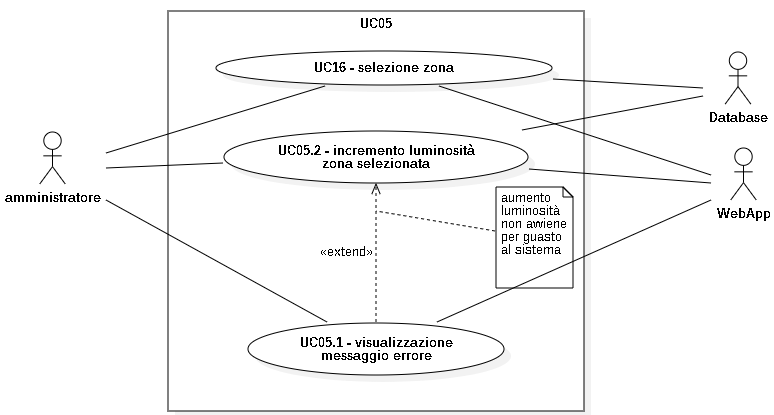
\includegraphics[scale=0.5]{UC05.png}

\subsection{UC06 - Rimozione area illuminata}
\textbf{Tipologia: obbligatorio} \\
L'amministratore vuole rimuovere un'area illuminata in quanto non viene più gestita dal sistema.
\begin{itemize}
	\item Attori primari: SuperAdmin, Admin
	\item Precondizioni: gli amministratori vogliono rimuovere un'area illuminata gestita tramite la webapp
	\item Postcondizioni: viene rimossa l'area e i relativi dispositivi presenti e non è più possibile effettuare le operazioni consentite.
\end{itemize}
\paragraph{Scenario Principale}
\begin{itemize}
	\item l'utente accede alla lista delle aree gestite
	\item l'utente rimuove l'area illuminata tramite l'apposito tasto
	\item l'area viene rimossa dal database 
	\item i lampioni e i sensori afferenti a tale area vengono eliminati a cascata dal database
\end{itemize}

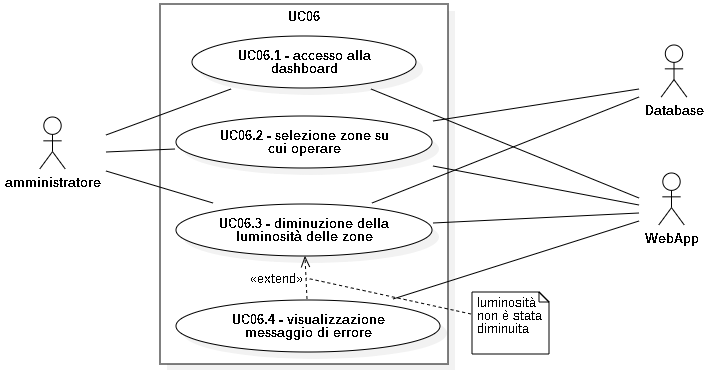
\includegraphics[scale=0.5]{UC06.png}

\subsection{UC07 - Modifica informazioni area illuminata}
\textbf{Tipologia: obbligatorio} \\
L'utente vuole modificare le informazioni di un'area illuminata, come ad esempio l'indirizzo ip di un sensore che è stato sostituito.
\begin{itemize}
	\item Attori primari: SuperAdmin, Admin
	\item Precondizioni: gli amministratori vogliono modificare le informazioni di un'area illuminata da gestire tramite la webapp
	\item Postcondizioni: vengono modificati i dettagli dell'area in questione ed è possibile effettuare le operazioni consentite dal software.
\end{itemize}
\paragraph{Scenario Principale}
\begin{itemize}
	\item l'utente accede alla lista delle aree gestite
	\item l'utente selezione l'area desiderata
	\item l'utente preme l'apposito pulsante di modifica
	\item l'utente può modificare i seguenti parametri:
		\begin{itemize}
			\item Nome città
			\item Zona geografica in cui si trova l'impianto di illuminazione
			\item Modalità di funzionamento
			\item luminosità in caso di assenza di rilevamenti
			\item luminosità in caso di rilevamenti
		\end{itemize}
	\item le informazioni aggiornate vengono salvate sul database
\end{itemize}
\paragraph{Estensioni} In caso di un errore nell'inserimento dei parametri nuovi nel DB, l'amministratore riceve un messaggio di errore.

\subsubsection{UC07.1 - Visualizzazione del messaggio d'errore in modalità di modifica}
\begin{itemize}
	\item Attore primario: SuperAdmin, Admin
	\item Precondizioni: L'attore primario ha modificato uno o più dettagli di un'area illuminata
	\item Post-condizioni: I dettagli non vengono modificati e l'utente visualizza un messaggio recante un messaggio di errore.
\end{itemize}

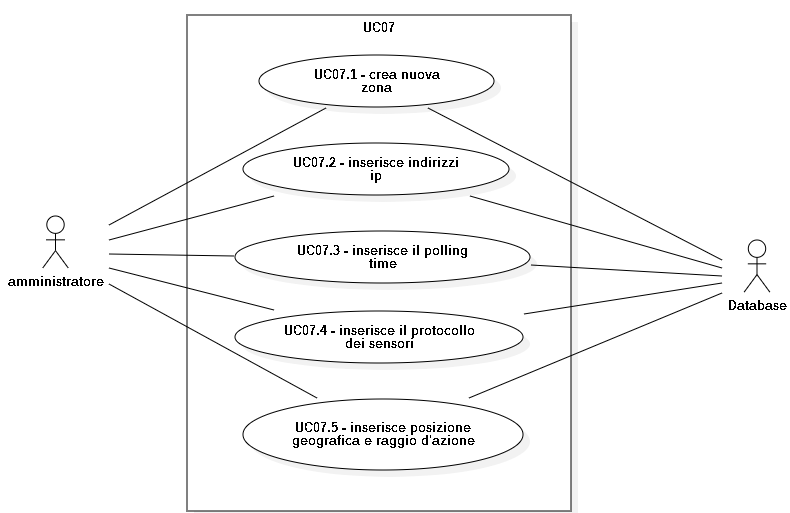
\includegraphics[scale=0.5]{UC07.png}

\subsection{UC08 - Inserimento nuovo sensore}
\textbf{Tipologia: obbligatorio}\\
L'amministratore vuole inserire un nuovo sensore che comanda l'aumento o la riduzione della luminosità di un'area gestita.
\begin{itemize}
	\item Attori primari: SuperAdmin, Admin
	\item Precondizioni: gli amministratori vogliono inserire un nuovo sensore a sistema per la rilevazione degli utenti stradali.\\
	 Per compiere quest'operazione è necessario essere in possesso delle seguenti informazioni: 
	\begin{itemize}
		\item area illuminata in cui il sensore è installato
		\item tipo di iterazione con il sensore: Push o Pull
		\item indirizzo IP
		\item polling time
		\item zona geografica di posizionamento del sensore
		\item raggio d'azione del dispositivo
	\end{itemize}
	\item Postcondizioni: il sensore viene inserito a sistema ed è possibile sfruttare il funzionamento automatico del sistema.
\end{itemize}
\paragraph{Scenario Principale}
\begin{itemize}
	\item l'utente accede ad un area illuminata
	\item l'utente preme il pulsante di inserimento di un sensore
	\item l'utente inserisce i dettagli richiesti dal form per l'inserimento
	\item l'utente preme salva
\end{itemize}
\paragraph{Estensioni} In caso di un errore nell'inserimento dei parametri nuovi,l'amministratore riceve un messaggio di errore.

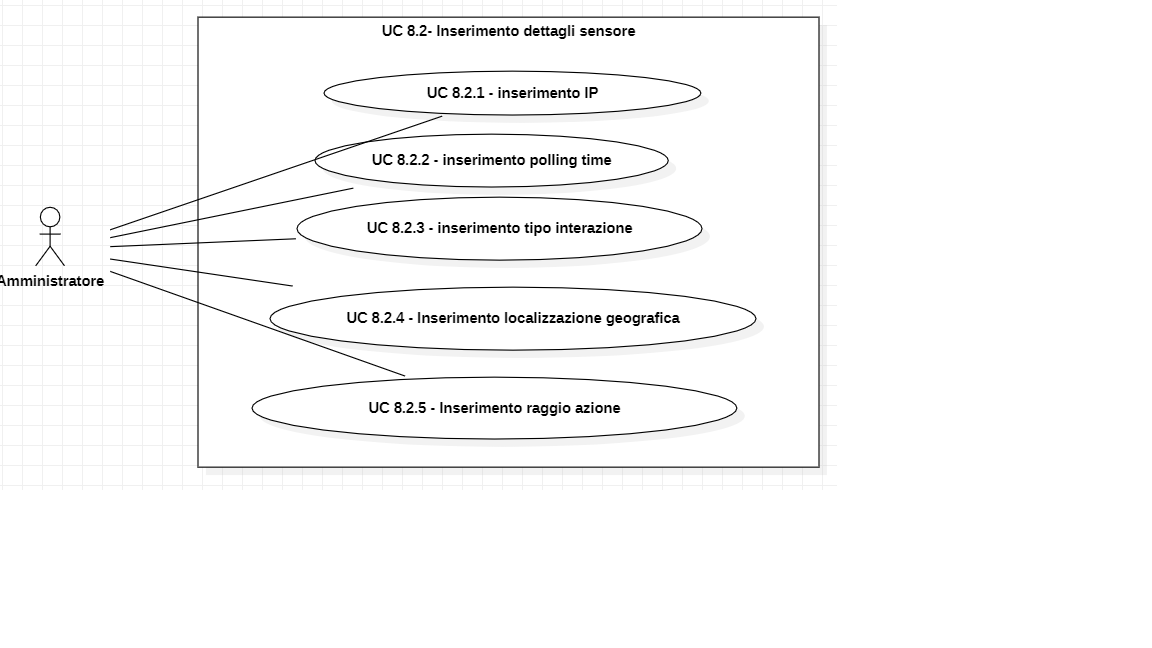
\includegraphics[scale=0.5]{UC08.png}

\subsection{UC09 - Rimozione sensore}
\textbf{Tipologia: obbligatorio}\\
L'amministratore vuole rimuovere un sensore che comanda l'aumento o la riduzione della luminosità di un'area gestita.
\begin{itemize}
	\item Attori primari: SuperAdmin, Admin
	\item Precondizioni: gli amministratori vogliono rimuovere un sensore dal sistema.
	\item Postcondizioni: non è più possibile aumentare o diminuire automaticamente la luminosità in una data area.
\end{itemize}
\paragraph{Scenario Principale}
\begin{itemize}
	\item l'utente accede ad un area illuminata
	\item l'utente preme il pulsante di rimozione di un sensore
	\item il sensore viene rimosso dal database
	\item l'utente riceve un messaggio di successo o di errore
\end{itemize}


\subsection{UC10 - Logout dal sistema}
\textbf{Tipologia: obbligatorio} \\
L'utente è riconosciuto come amministratore e vuole effettuare il logout dal sistema.
\begin{itemize}
	\item Attori primari: SuperAdmin, Admin
	\item Precondizioni: l'amministratore ha accesso al sistema per poterlo gestire
	\item Postcondizioni: l'utente viene disconnesso e non può più operare, ma rimane nella lista degli amministratori.
\end{itemize}
\paragraph{Scenario Principale}
\begin{itemize}
	\item l'utente ha accesso al sistema
	\item l'utente preme il pulsante di logout
	\item viene effettuata la disconnessione ed è necessario reinserire le credenziali per operare nuovamente
\end{itemize}


\subsection{UC11 - Visualizzazione elenco aree illuminate}
\textbf{Tipologia: obbligatorio} \\
L'utente autorizzato vuole avere una panoramica delle aree illuminate
\begin{itemize}
	\item Attori primari: SuperAdmin, Admin
	\item Precondizioni: l'utente è un amministratore e vuole avere una panoramica sulla luminosità e sullo stato del sistema.
	\item Postcondizioni: l'amministratore visualizza la lista delle aree e può interagire
\end{itemize}
\paragraph{Scenario Principale}
\begin{itemize}
	\item l'utente preme il pulsante che fornisce la panoramica del sistema
	\item l'elenco delle aree a sistema viene reperito dal database
	\item viene visualizzato l'elenco delle aree illuminate
\end{itemize}


\subsection{UC12 - Inserimento di un impianto nella sezione guasti}
\textbf{Tipologia: obbligatorio} \\
L'amministratore rileva un guasto e inserisce manualmente l'impianto nell'elenco dei sistemi con guasti.
\begin{itemize}
	\item Attori primari: SuperAdmin, Admin
	\item Precondizioni: un sensore rileva una discrepanza tra luminosità rilevata e quella impostata in un'impianto gestito.
	\item Postcondizioni: l'amministratore inserisce l'area nell'elenco dei guasti
\end{itemize}
\paragraph{Scenario Principale}
\begin{itemize}
	\item l'utente preme il pulsante che fornisce la panoramica del sistema
	\item viene visualizzato l'elenco delle aree illuminate
	\item viene rilevata una discrepanza tra luminosità misurata e quella impostata. Viene segnalata graficamente la presenza del guasto.
	\item l'amministratore inserisce l'impianto nell'elenco dei guasti
	\item viene aggiornata la tabella dei guasti nel database
\end{itemize}

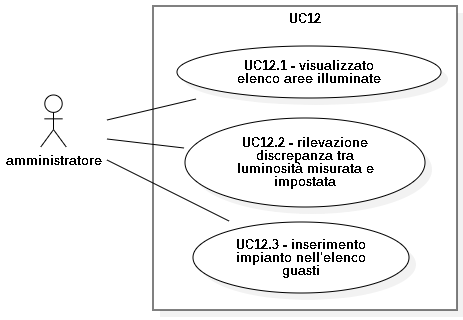
\includegraphics[scale=0.5]{UC12.png}

\subsection{UC13 - Rimozione di un impianto dalla sezione guasti}
\textbf{Tipologia: obbligatorio} \\
L'impianto è marcato come guasto, ma il malfunzionamento è stato risolto.
\begin{itemize}
	\item Attori primari: Amministratore
	\item Precondizioni: l'impianto con un guasto viene sistemato
	\item Postcondizioni: l'amministratore rimuove l'area in questione dall'elenco dei guasti
\end{itemize}
\paragraph{Scenario Principale}
\begin{itemize}
	\item l'amministratore accede alla lista degli impianti guasto
	\item l'utente seleziona l'impianto su cui è stata eseguita la manutenzione
	\item l'utente preme il pulsante di cancellazione dall'elenco
	\item l'impianto viene rimosso dalla sezione guasti aperti
	\item nella webapp l'impianto appare nuovamente come funzionante
\end{itemize}


\subsection{UC14 - Visualizzazione dettagliata di un'area}
\textbf{Tipologia: obbligatorio} \\
L'amministratore vuole conoscere in dettaglio le impostazioni di un'area.
\begin{itemize}
	\item Attori primari: SuperAdmin, Admin
	\item Precondizioni: l'amministratore vuole sapere lo stato di un'area e la luminosità pre-impostata
	\item Postcondizioni: l'utente ottiene le informazioni desiderate
\end{itemize}
\paragraph{Scenario Principale}
\begin{itemize}
	\item l'utente preme il pulsante che fornisce la panoramica delle aree
	\item l'utente sceglie l'area desiderata
	\item vengono visualizzate tutte le informazioni dell'area di interesse
\end{itemize}

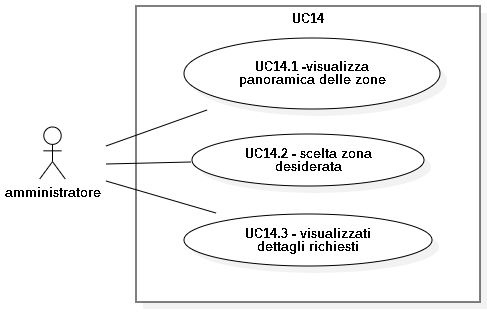
\includegraphics[scale=0.5]{UC14.png}

\subsection{UC15 - Visualizzazione dettagliata di un lampione}
\textbf{Tipologia: obbligatorio} \\
L'amministratore vuole conoscere in dettaglio la luminosità di un lampione.
\begin{itemize}
	\item Attori primari: SuperAdmin, Admin
	\item Precondizioni: l'amministratore vuole sapere lo stato e le impostazioni di un lampione
	\item Postcondizioni: l'utente visualizza le impostazioni del lampione
\end{itemize}
\paragraph{Scenario Principale}
\begin{itemize}
	\item l'utente preme il pulsante che fornisce la panoramica delle aree
	\item l'utente sceglie l'area desiderata
	\item l'utente preme il pulsante panoramica lampioni
	\item vengono fornite le info dettagliate per ogni lampione dell'area
\end{itemize}

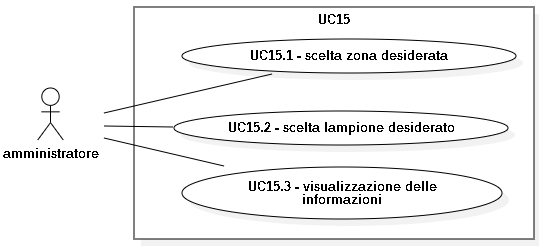
\includegraphics[scale=0.5]{UC15.png}

\subsection{UC16 - Inserimento di un lampione}
\textbf{Tipologia: obbligatorio}\\
L'amministratore vuole inserire un nuovo lampione all'interno di un'area gestita.
\begin{itemize}
	\item Attori primari: SuperAdmin, Admin
	\item Precondizioni: gli amministratori vogliono inserire un nuovo lampione a sistema.\\
	 Per compiere quest'operazione è necessario essere in possesso delle seguenti informazioni: 
	\begin{itemize}
		\item tipo di iterazione con il lampione: Push o Pull
		\item indirizzo IP
		\item polling time
		\item luminosità manuale
		\item area illuminata di afferenza
	\end{itemize}
	\item Postcondizioni: il lampione è inserito a sistema e può essere comandato.
\end{itemize}
\paragraph{Scenario Principale}
\begin{itemize}
	\item l'utente accede ad un area illuminata
	\item l'utente preme il pulsante di inserimento di un lampione
	\item l'utente inserisce i dettagli richiesti dal form per l'inserimento
	\item l'utente preme salva
	\item il lampione viene aggiunto nel database nell'area di competenza
	\item l'utente riceve un messaggio di successo o di errore
\end{itemize}


\subsection{UC17 - Rimozione lampione}
\textbf{Tipologia: obbligatorio}\\
L'amministratore vuole rimuovere un lampione all'interno dell'area gestita.
\begin{itemize}
	\item Attori primari: SuperAdmin, Admin
	\item Precondizioni: gli amministratori vogliono rimuovere un lampione a sistema.\\
	\item Postcondizioni: il lampione non è più comandabile e non fa più parte dell'area.
\end{itemize}
\paragraph{Scenario Principale}
\begin{itemize}
	\item l'utente accede ad un area illuminata
	\item l'utente selezione il lampione desiderato
	\item l'utente preme il pulsante di modifica
	\item l'utente preme elimina
	\item il lampione viene rimosso dal database
	\item l'utente riceve un messaggio di errore o di successo
\end{itemize}


\subsection{UC18 - Consultazione elenco aree con guasti}
\textbf{Tipologia: obbligatorio}\\
Il manutentore vuole consultare la lista delle aree con dei malfunzionamenti per sapere dove intervenire.
\begin{itemize}
	\item Attori primari: manutentore, Admin e SuperAdmin
	\item Precondizioni: un utente vuole sapere quali aree presentano dei guasti.\\
	\item Postcondizioni: l'utente ottiene la lista delle aree in cui è stato rilevato un malfunzionamento.
\end{itemize}
\paragraph{Scenario Principale}
\begin{itemize}
	\item l'utente selezione il pulsante per la panoramica dei guasti
	\item la tabella corrispondente viene reperita dal database
	\item vengono visualizzati i guasti non risolti e lo storico di quelli risolti
\end{itemize}


\subsection{UC19 - Apertura ticket}
\textbf{Tipologia: obbligatorio}\\
L'amministratore apre un ticket per un guasto rilevato
\begin{itemize}
	\item Attori primari: Admin
	\item Precondizioni: è stato rilevato un guasto in un'area illuminata.
	\item Postcondizioni: un apposito ticket è stato creato e presenta i dettagli utili al manutentore.
\end{itemize}
\paragraph{Scenario Principale}
\begin{itemize}
	\item viene rilevato un guasto
	\item l'Admin crea il nuovo ticket
	\item il ticket è visualizzabile dal manutentore
\end{itemize}


\subsection{UC20 - Chiusura ticket}
\textbf{Tipologia: obbligatorio}\\
L'amministratore chiude un ticket del un guasto sistemato
\begin{itemize}
	\item Attori primari: Admin
	\item Precondizioni: è stata fatta la dovuta manutenzione
	\item Postcondizioni: il ticket che era stato creato è stato archiviato. 
\end{itemize}
\paragraph{Scenario Principale}
\begin{itemize}
	\item il guasto rilevato viene sistemato
	\item l'Admin chiude il ticket precedentemente creato
	\item il titcket viene archiviato
\end{itemize}

\subsection{UC20 - Visualizzazione lista lampioni area}
\textbf{Tipologia: obbligatorio}\\
L'amministratore vuole vedere la lista dei lampioni di un'area
\begin{itemize}
	\item Attori primari: Admin
	\item Precondizioni: l'amministratore vuole visualizzare tutti i lampioni che afferiscono ad un'area
	\item Postcondizioni: l'amministratore visualizza le informazioni richieste. 
\end{itemize}
\paragraph{Scenario Principale}
\begin{itemize}
	\item l'amministratore seleziona l'area di interesse
	\item l'Admin preme il pulsante per la visualizzazione della lista dei lampioni
	\item vengono visualizzate le informazioni richieste
\end{itemize}

\subsection{UC21 - Visualizzazione lista sensori area}
\textbf{Tipologia: obbligatorio}\\
L'amministratore vuole vedere la lista dei sensori di un'area
\begin{itemize}
	\item Attori primari: Admin
	\item Precondizioni: l'amministratore vuole visualizzare tutti i sensori che afferiscono ad un'area
	\item Postcondizioni: l'amministratore visualizza le informazioni richieste. 
\end{itemize}
\paragraph{Scenario Principale}
\begin{itemize}
	\item l'amministratore seleziona l'area di interesse
	\item l'Admin preme il pulsante per la visualizzazione della lista dei sensori
	\item vengono visualizzate le informazioni richieste
\end{itemize}

\subsection{UC22 - Modifica lampione}
\textbf{Tipologia: obbligatorio} \\
L'utente vuole modificare le informazioni di un lampione.
\begin{itemize}
	\item Attori primari: SuperAdmin, Admin
	\item Precondizioni: gli amministratori vogliono modificare le informazioni di un lampione da gestire tramite la webapp
	\item Postcondizioni: vengono modificati i dettagli del lampione in questione.
\end{itemize}
\paragraph{Scenario Principale}
\begin{itemize}
	\item l'utente accede alla lista delle aree gestite
	\item l'utente preme il pulsante per visualizzare la lista dei lampioni
	\item l'utente sceglie il lampione desiderato
	\item l'utente preme il pulsante di modifica
	\item l'utente può modificare i seguenti parametri:
		\begin{itemize}
			\item IP
			\item tipo interazione
			\item luminosità manuale
		\end{itemize}
	\item le informazioni aggiornate vengono salvate sul database
\end{itemize}

\subsection{UC22 - Modifica sensore}
\textbf{Tipologia: obbligatorio} \\
L'utente vuole modificare le informazioni di un sensore.
\begin{itemize}
	\item Attori primari: SuperAdmin, Admin
	\item Precondizioni: gli amministratori vogliono modificare le informazioni di un sensore da gestire tramite la webapp
	\item Postcondizioni: vengono modificati i dettagli del sensore in questione.
\end{itemize}
\paragraph{Scenario Principale}
\begin{itemize}
	\item l'utente accede alla lista delle aree gestite
	\item l'utente preme il pulsante per visualizzare la lista dei sensori
	\item l'utente sceglie il sensore desiderato
	\item l'utente preme il pulsante di modifica
	\item l'utente può modificare i seguenti parametri:
		\begin{itemize}
			\item IP
			\item polling time
			\item tipo interazione
			\item raggio di azione
		\end{itemize}
	\item le informazioni aggiornate vengono salvate sul database
\end{itemize}


\section{UC Desiderabili}

\subsection{UC23 - Visualizzazione lista ticket}
\textbf{Tipologia: desiderabile}\\
Il manutentore vuole consultare i dettagli di un guasto
\begin{itemize}
	\item Attori primari: manutentore
	\item Precondizioni: il manutentore vuole sapere ulteriori dettagli sull'area da operare.
	\item Postcondizioni: il ticket fornisce delle informazioni aggiuntive.
\end{itemize}
\paragraph{Scenario Principale}
\begin{itemize}
	\item il manutentore visualizza i vari guasti
	\item il manutentore sceglie il guasto su cui intervenire
	\item visualizza il ticket che mostrerà ulteriori informazioni
\end{itemize}


\subsection{UC24 - Primo accesso al sistema senza credenziali}
\textbf{Tipologia: desiderabile.} \\
L'utente vuole poter operare come amministratore ma non ha ancora ottenuto le credenziali necessarie all'accesso.
\begin{itemize}
	\item Attori primari: Nuovi Admin
	\item Precondizioni: i nuovi amministratori vorrebbero poter accedere al sistema, ma non sono ancora autorizzati
	\item Postcondizioni: I SuperAmministratori, dopo essere stata contattati dagli amministratori interessati, forniscono le credenziali per l'accesso al sistema.
\end{itemize}
\paragraph{Scenario Principale}
\begin{itemize}
	\item l'utente contatta via mail il servizio clienti di del gestore del sisitema
	\item il superamministratore del sistema fornisce le credenziali
	\item l'utente viene impostato come amministratore
	\item l'utente effettua l'accesso
	\item l'utente riceve una conferma di avvenuto accesso e può operare nella dashboard
\end{itemize}


\subsection{UC25 - Consultazione manuale Lumos Minima}
\textbf{Tipologia: desiderabile}\\
L'utente non sa come funziona il sistema o come eseguire un'operazione specifica e vuole approfondire questi aspetti.
\begin{itemize}
	\item Attori primari: SuperAdmin, Admin, Manutentori
	\item Precondizioni: l'amministratore o il manutentore usa il sistema e vorrebbe avere una panoramica dettagliata sul suo funzionamento.
	\item Postcondizioni: l'utente consulta il manuale d'uso
\end{itemize}
\paragraph{Scenario Principale}
\begin{itemize}
	\item L'utente visualizza la dashboard
	\item l'utente clicca l'apposito bottone per visualizzare il manuale
	\item viene aperta una nuova finestra del browser che mostra il manuale utente sottoforma di PDF
\end{itemize}


\subsection{UC26 - Configurazione iniziale delle impostazioni di una nuova area illuminata}
\textbf{Tipologia: desiderabile} \\
Per ogni area illuminata inserita a sistema vengono fornite delle impostazioni di default che permettono il corretto funzionamento del sistema senza intraprendere azioni aggiuntive.
\begin{itemize}
	\item Attori primari: SuperAdmin, Admin
	\item Precondizioni: l'amministratore accede al sistema e inserisce una nuova area illuminata.
	\item Postcondizioni: la nuova area viene settata con delle impostazioni standard, senza richiedere ulteriori azioni
\end{itemize}
\paragraph{Scenario Principale}
\begin{itemize}
	\item l'utente aggiunge una nuova area illuminata
	\item vengono applicate le impostazioni di default, come la luminosità minima e massima
	\item tutti i lampioni dell'area vengono tarati con queste impostazioni.
\end{itemize}


\section{Requisiti}
\subsection{Funzionali}
 \begin{tabularx}{\linewidth}{|>{\hsize=0.6\hsize}X|>{\hsize=1.8\hsize}X|>{\hsize=1\hsize}X|>{\hsize=0.6\hsize}X|}
% \begin{xltabular}{200pt}{|c|X|c|X|}
\hline
\textbf{Requisito} & \textbf{Descrizione} & \textbf{Classificazione} & \textbf{Fonti} \\
\hline
\endfirsthead
\hline
\textbf{Requisito} & \textbf{Descrizione} & \textbf{Classificazione} & \textbf{Fonti} \\
\hline
\endhead
\hline
\endfoot
RF1	 & L'utente deve poter fare il login al sistema	 & Obbligatorio & UC1 \\
\hline				
RF2	 & L'utente visualizza lo stato del sistema	 & Obbligatorio & UC2 \\
\hline				
RF3	 & L'utente deve poter aumentare la luminosità di un'area & Obbligatorio & UC3 \\
\hline				
RF4	 & Il sistema deve visualizzare un messaggio d'errore se non si è potuto aumentare la luminosità & Obbligatorio	& UC3.1 \\
\hline	
RF5 & L'utente deve poter vedere l'elenco delle aree illuminate	 & Obbligatorio & UC12.1, UC11 \\
\hline
RF6 & L'utente deve poter vedere l'elenco delle aree & Obbligatorio & UC14.1 \\
\hline
RF7	 & L'utente deve poter selezionare le aree su cui operare & Obbligatorio & UC4.2, UC14.2,  \\
\hline	
RF8	 & L'utente deve poter diminuire la luminosità di un'area & Obbligatorio & UC4 \\
\hline				
RF10	 & L'utente deve poter accedere alla dashboard & Obbligatorio & UC4.1 \\
\hline										
RF11	 & Il sistema deve visualizzare un messaggio d'errore nel caso l'operazione di diminuzione della luminosità non fosse andata a buon fine & Obbligatorio & UC4.3, UC4.4 \\
\hline				
RF12	 & L'utente deve poter diminuire la luminosità & Obbligatorio & UC4 \\
\hline				
RF13	 & L'utente deve poter inserire una nuova area illuminata & Obbligatorio & UC5 \\
\hline				
RF14	 & L'utente deve poter rimuovere un area illuminata & Obbligatorio & UC6.2 \\
\hline				
RF15	 & L'utente deve poter accedere alla lista delle aree gestite & Obbligatorio & UC6.1 \\
\hline				
RF16	 & L'utente deve poter modificare le informazioni di un'area illuminata & Obbligatorio & UC7 \\
\hline				
RF17	 & Il sistema mostra un messaggio di notifica una volta effettuata la modifica ad un area illuminata & Obbligatorio	& UC7.3 \\
\hline				
RF18	 & L'utente deve poter inserire un nuovo sensore in una area illuminata & Obbligatorio & Capitolato, UC8 \\
\hline				
RF19	 & L'utente deve poter accedere all'area illuminata & Obbligatorio & Capitolato, UC8.1 \\
\hline 				
RF20	 & L'utente deve poter rimuovere un sensore da un'area illuminata & Obbligatorio & UC9 \\
\hline				
RF21	 & L'utente deve poter fare il logout dal sistema & Obbligatorio & Capitolato UC10 \\
\hline										
RF22	 & L'utente deve poter inserire un impianto nell'elenco dei guasti & Obbligatorio & UC12 \\
\hline				
RF23	 & L'utente deve poter rimuovere un impianto dall'elenco dei guasti & Obbligatorio & UC13 \\
\hline				
RF24	 & L'utente deve poter visualizzare i dettagli di un'area & Obbligatorio & UC14 \\
\hline				
RF25	 & L'utente deve poter selezionare un lampione & Obbligatorio & UC15.2\\
\hline				
RF26	 & L'utente deve poter visualizzare i dettagli di un lampione & Obbligatorio & UC15\\
\hline				
RF27	 & L'utente deve poter inserire un nuovo lampione all'interno di un'area illuminata & Obbligatorio & UC16 \\
\hline				
RF28	 & L'utente deve poter rimuovere un lampione all'interno di un'area illuminata & Obbligatorio & UC17 \\
\hline				
RF29	 & L'utente deve poter visualizzare l'elenco delle aree illuminate con dei malfunzionamenti & Obbligatorio & UC18 \\
\hline				
RF30	 & L'amministratore deve poter aprire una nuova segnalazione di un guasto tramite un ticket & Obbligatorio & UC19 \\
\hline				
RF31	 & L'amministratore deve poter chiudere il ticket dopo aver fatto la dovuta manutenzione & Obbligatorio & UC20 \\
\hline				
RF32	 & Il manutentore deve poter visualizzare i dettagli aggiuntivi di un guasto forniti dal ticket & Desiderabile & UC21 \\
\hline				
RF33	 & L'utente non amministratore riceve le credenziali da amministratore da un superamministratore & Desiderabile & UC22 \\
\hline				
RF34	 & L'utente consulta il manuale Lumos Minima & Desiderabile & UC23 \\
\hline				
RF35	 & Le nuove aree illuminate appena inserite hanno un setup standard & Desiderabile & UC24 \\
\hline				
\end{tabularx}


\subsection{Qualità}
\begin{tabular}{ |p{1.8cm}|p{5.2cm}|p{3cm}| p{2cm}| }
\hline
Requisito& Descrizione &Classificazione &Fonti \\
\hline
RQ1 & La webapp deve essere sviluppata seguendo le regole descritte nel documento Norme di progetto & Obbligatorio & Capitolato \\
RQ2 & Devono essere sviluppati dei test con una copertura minima dell'80\% e correlati di report & Obbligatorio & Capitolato\\
RQ3 & Deve essere prodotto un documento sulle scelte implementative e progettuali & Obbligatorio & Capitolato \\
RQ4 & Deve essere prodotto un documento sui problemi aperti e sulle eventuali soluzioni da esplorare & Obbligatorio & Capitolato \\
RQ5 & Fornire un’analisi rispetto al carico massimo supportato in numero di dispositivi e di quale sarebbe il servizio cloud più adatto per supportarlo analizzando prezzo, stabilità del servizio ed assistenza.  &  Facoltativo & Capitolato \\
\hline

\end{tabular}
\subsection{Sistemi Operativi}
Siccome il prodotto da sviluppare è una webapp da eseguire su browser non è stato individuato nessun requisito sui sistemi operativi.
\subsection{Prestazionali}
L'azienda richiede che la webApp impegni al massimo 1GB di RAM e 2 CPU.
\end{document}
